\section{Pipeline}

Real world reconstruction from scan data is a step by step process:

\begin{itemize}
\item Scanning and scans alignment produce a point set with or without normals (not covered by \cgal)
\item Outlier removal (if reconstruction method does not support outliers)
\item Point set simplification
\item Smoothing (if reconstruction method does not support noise)
\item Normal estimation and orientation (if not provided by scanner)
\item Surface reconstruction
\end{itemize}

This package provides algorithms for each step above.

A GUI demo (Windows only) allows to test each algorithm.

% Insert image pipeline.jpg/eps
\begin{center}
    \label{Surface_reconstruction_3-fig-pipeline}
    % Image
    \begin{ccTexOnly}
        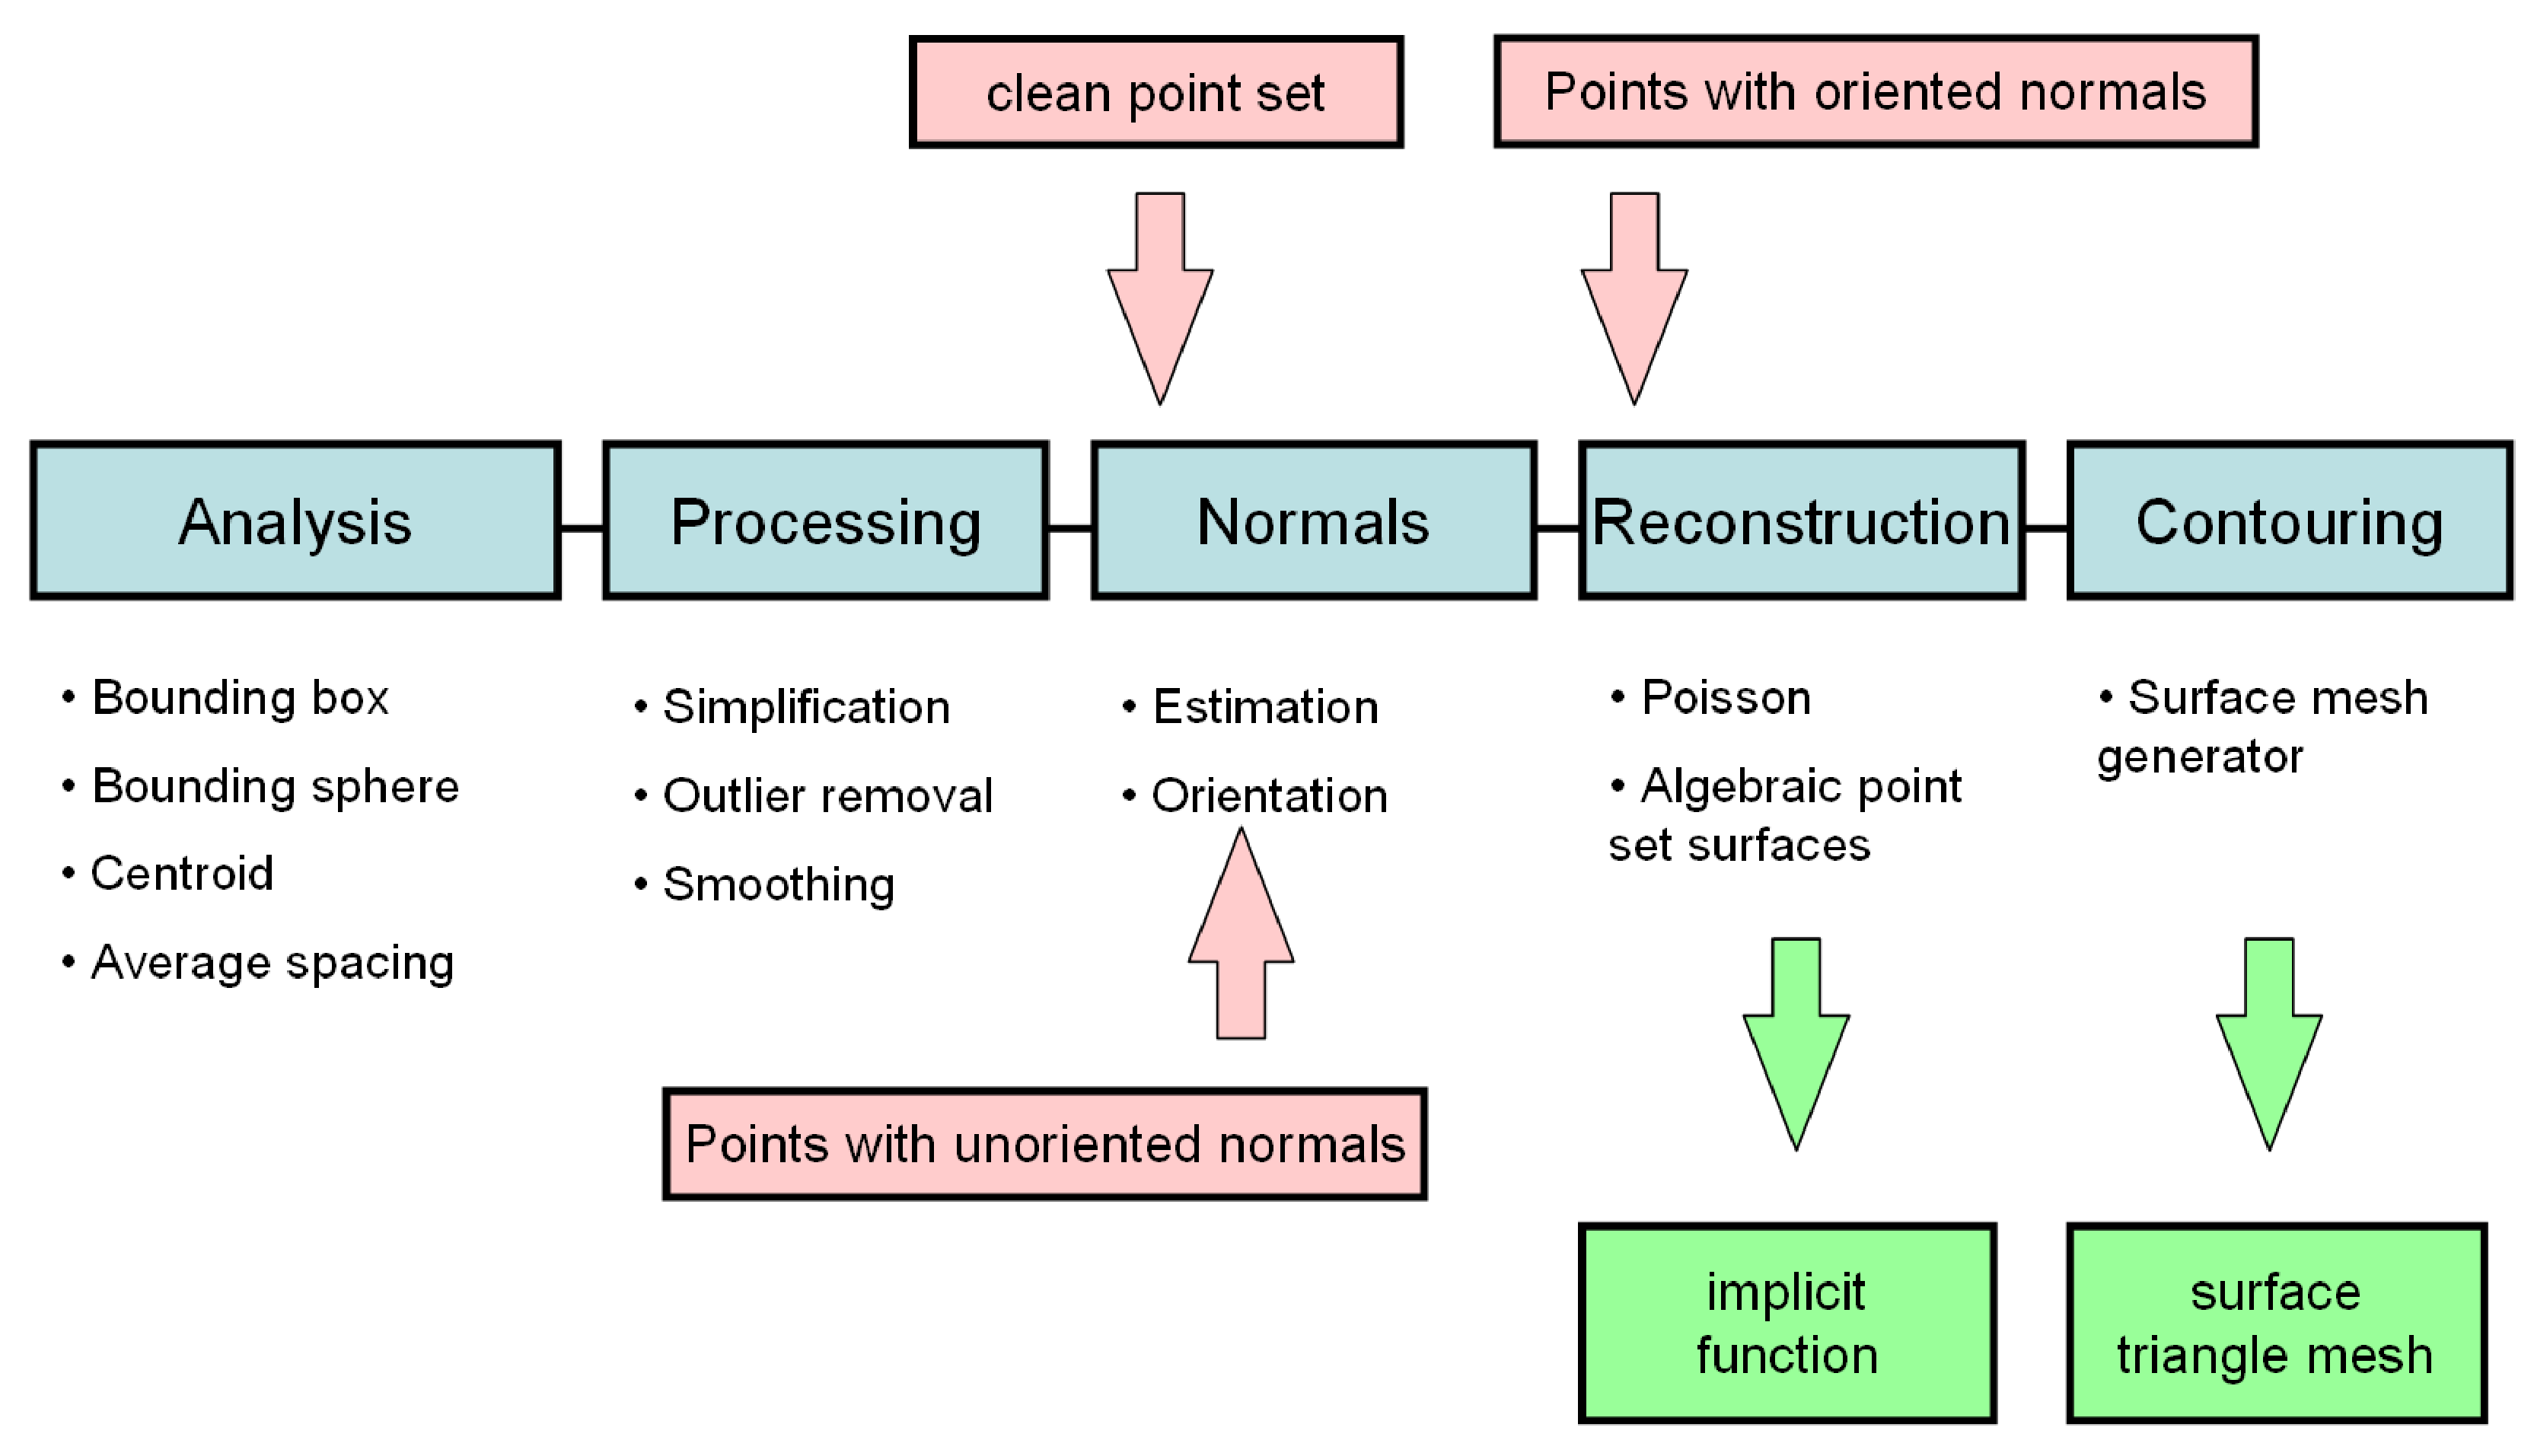
\includegraphics[width=1.0\textwidth]{Surface_reconstruction_3/pipeline} % omit .eps suffix
    \end{ccTexOnly}
    \begin{ccHtmlOnly}
        <img width="70%" border=0 src="./pipeline.jpg"><P>
    \end{ccHtmlOnly}
    % Title
    \begin{figure}[h]
        \caption{Reconstruction pipeline}
    \end{figure}
\end{center}


\subsection{Input}

Functions and classes of this package expect as input and output parameters range iterators over:

\begin{itemize}
\item 3D points
\item Normals (orientable 3D vectors)
\item 3D points with unoriented normals
\item 3D points with oriented normals
\end{itemize}

We provide several models of points and normals concepts, with different speed/space trade-offs:

\begin{itemize}
\item \ccRefIdfierPage{CGAL::Point_3<GeomTraits>} \\
\cgal\ 3D position.
\item \ccRefIdfierPage{CGAL::Vector_3<GeomTraits>} \\
\cgal\ 3D vector.
\item \ccRefIdfierPage{CGAL::Lightweight_vector_3<GeomTraits>} \\
3D vector allocated only if not (0,0,0).
\item \ccRefIdfierPage{CGAL::Orientable_normal_3<GeomTraits>} \\
Normal (oriented or not).
Inherits from \ccc{Vector_3<GeomTraits>} and contains an "is normal oriented?" flag.
\item \ccRefIdfierPage{CGAL::Point_with_normal_3<GeomTraits, Normal_3>} \\
3D position + normal.
\end{itemize}

For convenience, we provide also functions to read point sets from standard file formats:

\begin{itemize}
\item XYZ
\item OFF
\end{itemize}

\ccRefIdfierPage{CGAL::surface_reconstruction_read_xyz}  \\
\ccRefIdfierPage{CGAL::surface_reconstruction_read_off_point_cloud}  \\

Example:

\ccIncludeExampleCode{Surface_reconstruction_3/surface_reconstruction_read_write_xyz_example.cpp}


\subsection{Analysis}

The purpose of the analysis stage is to compute parameters for the next stages algorithms.

\begin{itemize}
\item Point set barycenter, bounding box, bounding sphere (provided by other \cgal\ packages).
\item Average spacing to the K nearest neighbors.
\end{itemize}

\ccc{CGAL::average_spacing_3()} computes the average spacing in a point set from the K nearest neighbors.

\ccRefIdfierPage{CGAL::centroid}  \\
\ccRefIdfierPage{CGAL::bounding_box}  \\
\ccRefIdfierPage{CGAL::average_spacing_3}  \\

Example:

\ccIncludeExampleCode{Surface_reconstruction_3/average_spacing_example.cpp}


\subsection{Processing}

\subsubsection{Outlier Removal}

\begin{itemize}
\item Outlier removal wrt average squared distance to the K nearest neighbors
\end{itemize}

\ccc{CGAL::outlier_removal_3()} deletes outliers in a point set. It sorts points
wrt average squared distance to the K nearest neighbors, then delete the worst ones.

\ccRefIdfierPage{CGAL::outlier_removal_3}  \\

% % Insert image outlier_removal.jpg/eps
% \begin{center}
%     \label{Surface_reconstruction_3-fig-outlier_removal}
%     % Image
%     \begin{ccTexOnly}
%         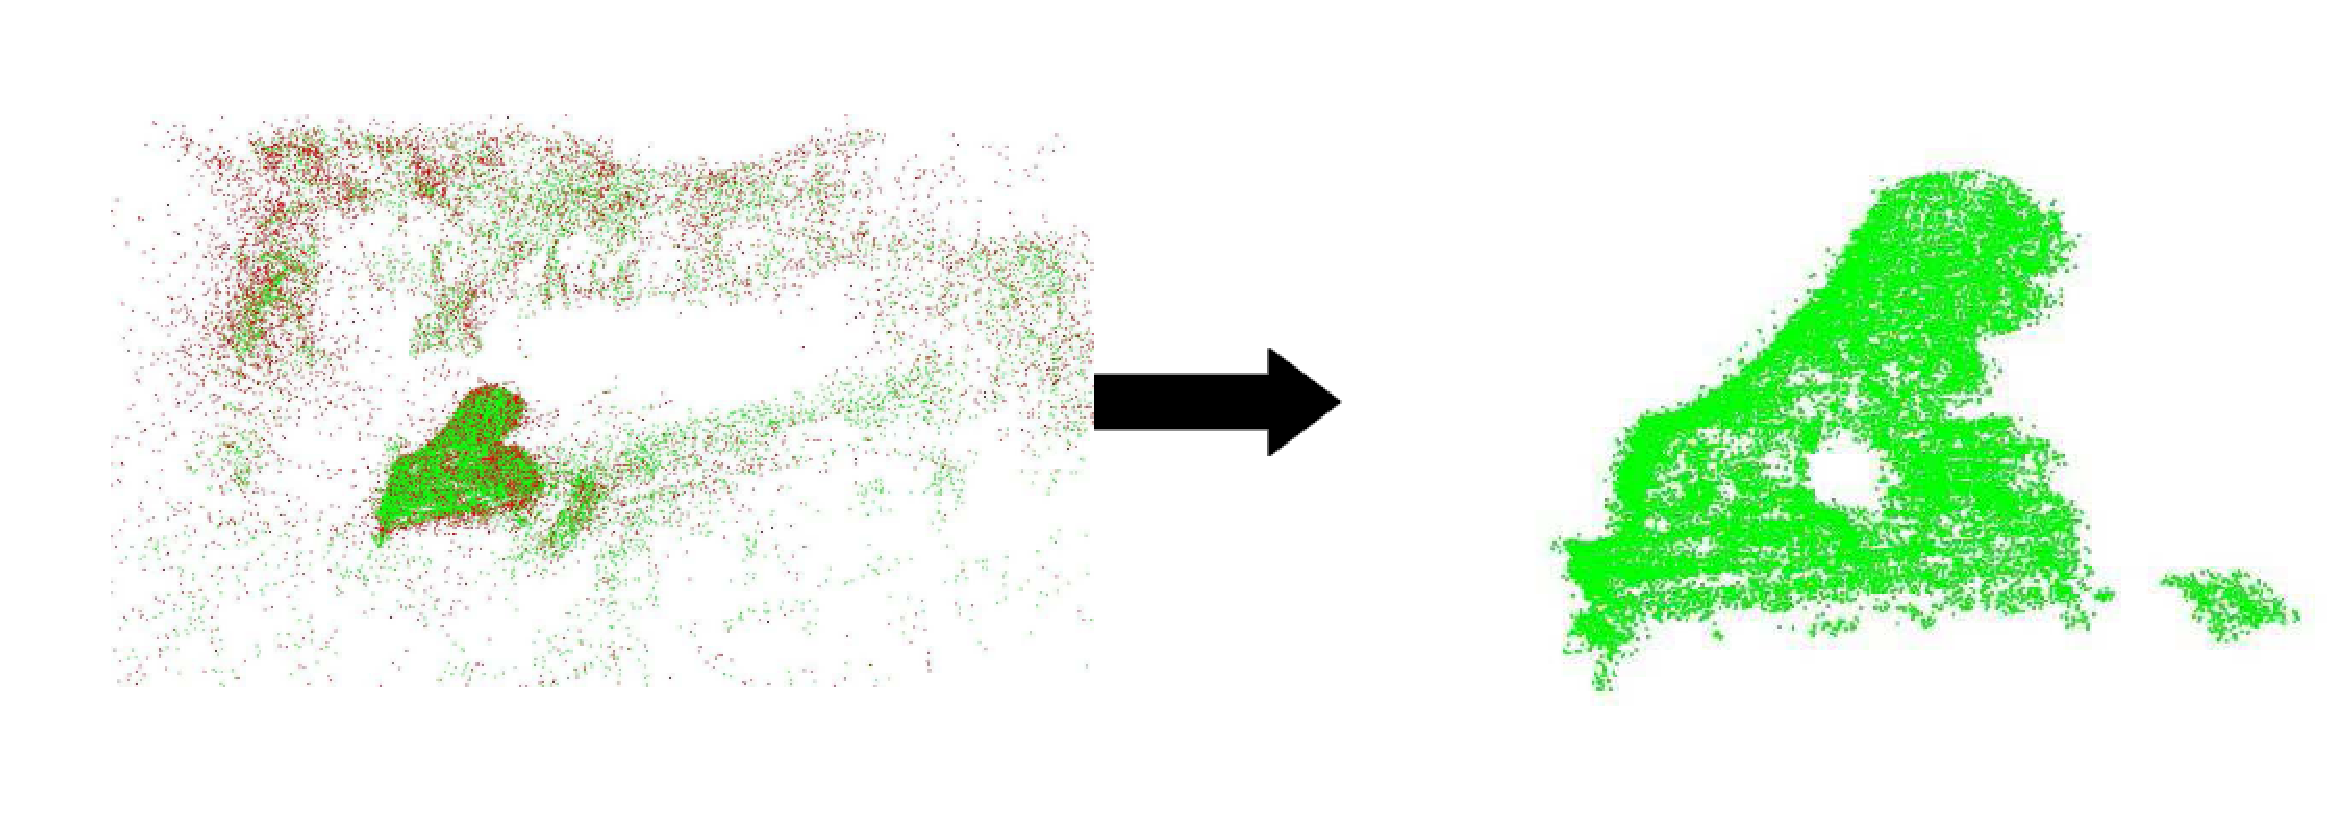
\includegraphics[width=0.9\textwidth]{Surface_reconstruction_3/outlier_removal} % omit .eps suffix
%     \end{ccTexOnly}
%     \begin{ccHtmlOnly}
%         <img width="90%" border=0 src="./outlier_removal.jpg"><P>
%     \end{ccHtmlOnly}
%     % Title
%     \begin{figure}[h]
%         \caption{Outlier removal}
%     \end{figure}
% \end{center}

Example:

\ccIncludeExampleCode{Surface_reconstruction_3/outlier_removal_example.cpp}


\subsubsection{Simplification}

\begin{itemize}
\item Point set simplification by clustering
\item Random point set simplification
\end{itemize}

\ccc{CGAL::merge_simplification_3()} merges close points of a point set: its merges points which belong to the same cell of a grid.

\ccc{CGAL::random_simplification_3()} deletes randomly points in a point set.

\ccRefIdfierPage{CGAL::merge_simplification_3}  \\
\ccRefIdfierPage{CGAL::random_simplification_3}  \\

% Insert image merge_simplification.jpg/eps
\begin{center}
    \label{Surface_reconstruction_3-fig-merge_simplification}
    % Image
    \begin{ccTexOnly}
        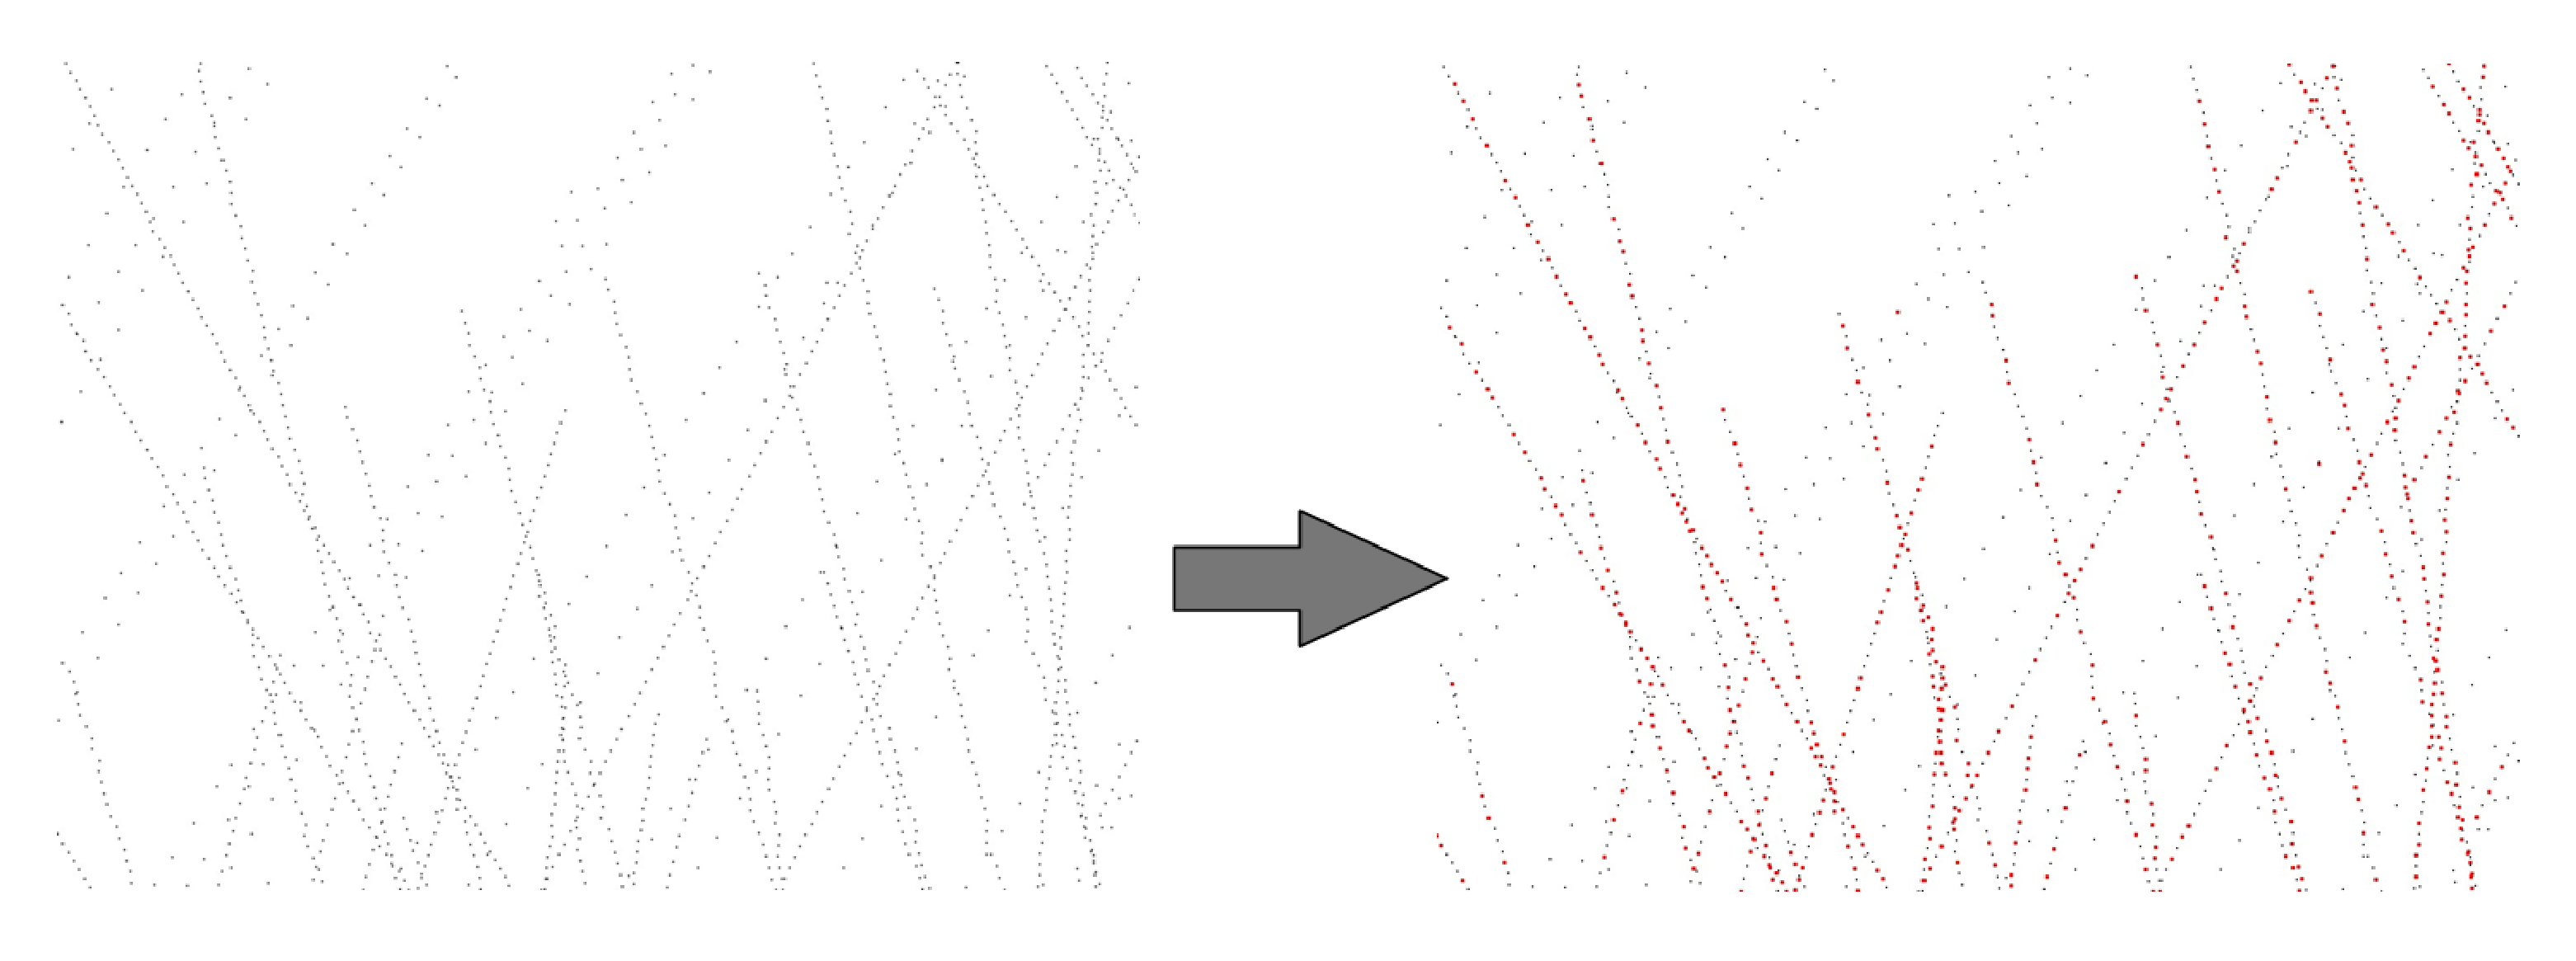
\includegraphics[width=0.7\textwidth]{Surface_reconstruction_3/merge_simplification} % omit .eps suffix
    \end{ccTexOnly}
    \begin{ccHtmlOnly}
        <img width="100%" border=0 src="../Surface_reconstruction_3/merge_simplification.jpg"><P>
    \end{ccHtmlOnly}
    % Title
    \begin{figure}[h]
        \caption{Point set simplification by clustering. Notice that points to be removed (in red) belong to tight dotted lines.}
    \end{figure}
\end{center}

Example:

\ccIncludeExampleCode{Surface_reconstruction_3/random_simplification_example.cpp}


\subsubsection{Smoothing}

\begin{itemize}
\item Smoothing via Jet fitting over the K nearest neighbors + reprojection
\end{itemize}

\ccRefIdfierPage{CGAL::jet_smoothing_3}  \\

% % Insert image jet_smoothing.jpg/eps
% \begin{center}
%     \label{Surface_reconstruction_3-fig-jet_smoothing}
%     % Image
%     \begin{ccTexOnly}
%         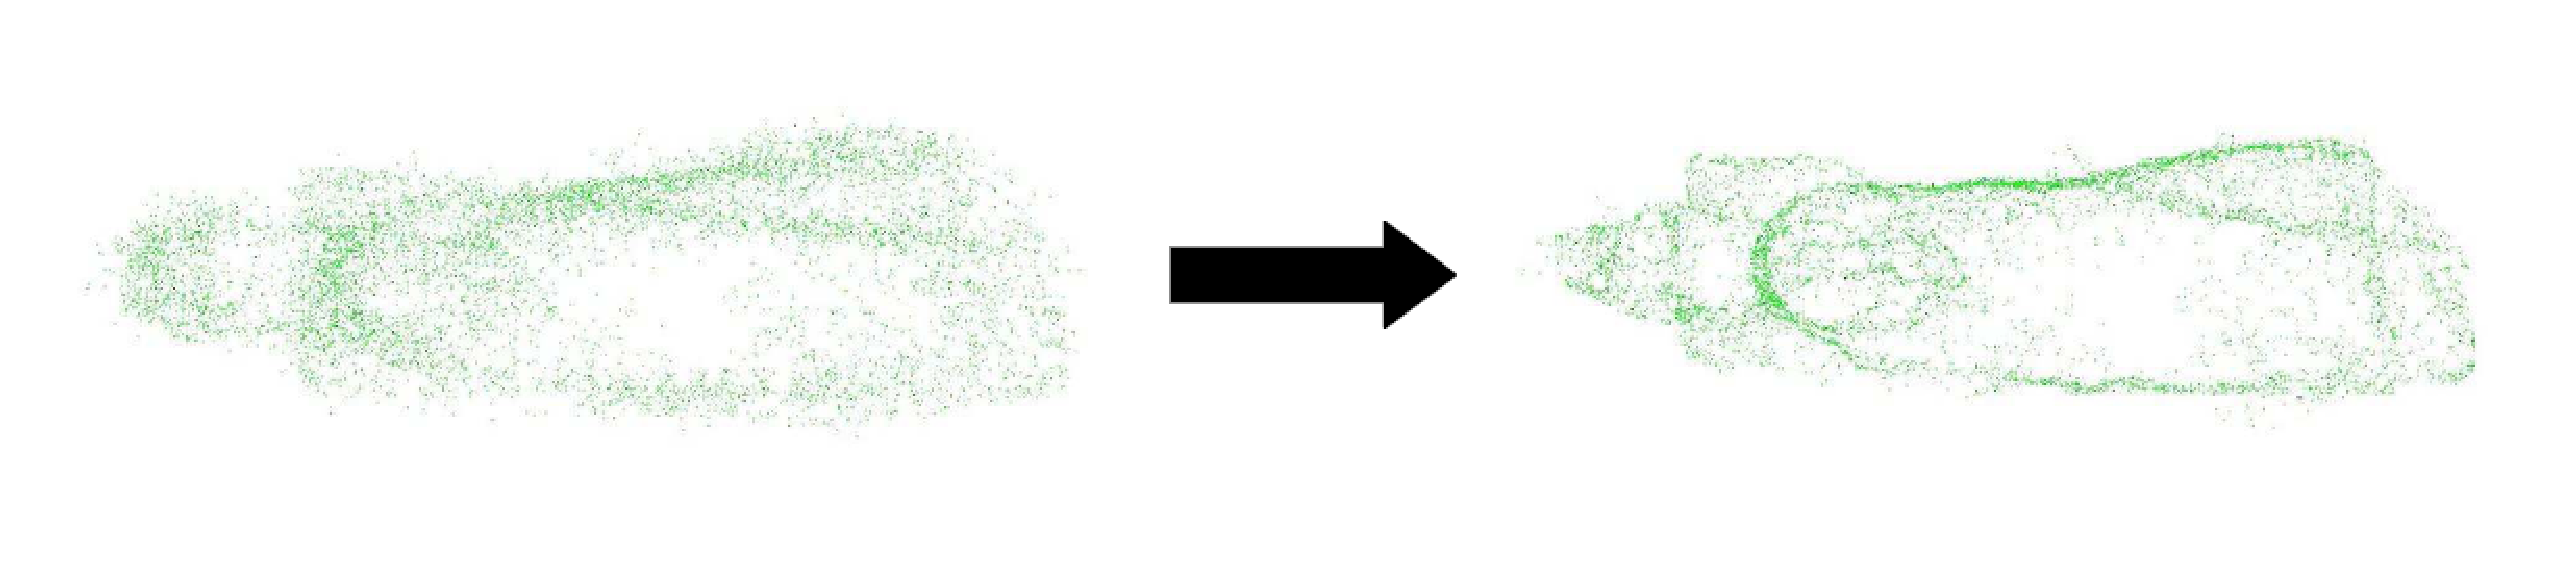
\includegraphics[width=1.0\textwidth]{Surface_reconstruction_3/jet_smoothing} % omit .eps suffix
%     \end{ccTexOnly}
%     \begin{ccHtmlOnly}
%         <img width="100%" border=0 src="./jet_smoothing.jpg"><P>
%     \end{ccHtmlOnly}
%     % Title
%     \begin{figure}[h]
%         \caption{Point set smoothing}
%     \end{figure}
% \end{center}

Example:

\ccIncludeExampleCode{Surface_reconstruction_3/jet_smoothing_example.cpp}


\subsubsection{Normal Estimation}

\begin{itemize}
\item Normal estimation by Principal Components Analysis over the K nearest neighbors
\item Normal estimation by Jet fitting over the K nearest neighbors
\end{itemize}

\ccc{CGAL::jet_normal_estimation()} estimates normals direction of a point set using jet fitting on the K nearest neighbors.
The default jet is a quadric.

\ccc{CGAL::pca_normal_estimation()} estimates normals direction of a point set using linear least squares fitting of a plane on the K nearest neighbors.

In both cases, the result is an unoriented normal vector for each input point.

\ccRefIdfierPage{CGAL::pca_normal_estimation}  \\
\ccRefIdfierPage{CGAL::jet_normal_estimation}  \\

% % Insert image pca_normal_estimation.jpg/eps
% \begin{center}
%     \label{Surface_reconstruction_3-fig-pca_normal_estimation}
%     % Image
%     \begin{ccTexOnly}
%         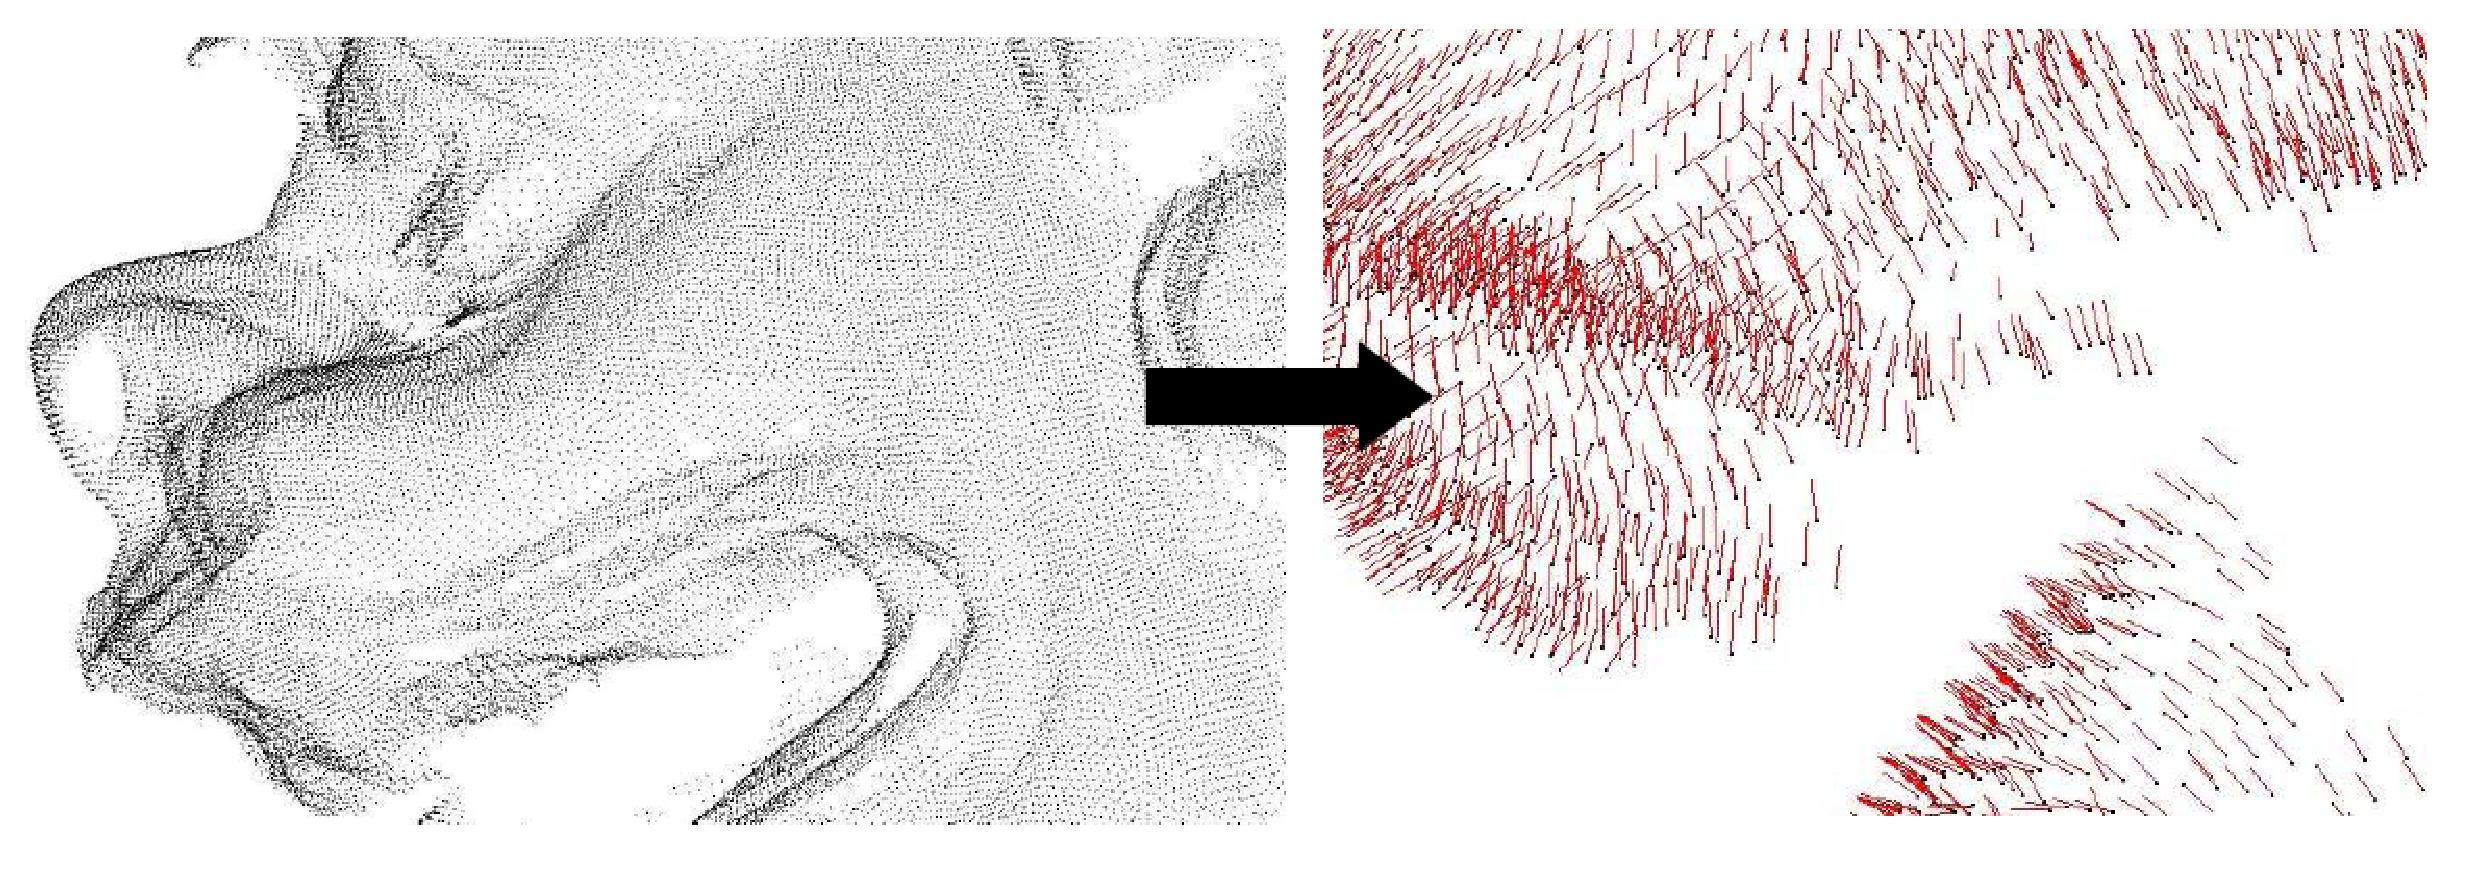
\includegraphics[width=0.9\textwidth]{Surface_reconstruction_3/pca_normal_estimation} % omit .eps suffix
%     \end{ccTexOnly}
%     \begin{ccHtmlOnly}
%         <img width="90%" border=0 src="./pca_normal_estimation.jpg"><P>
%     \end{ccHtmlOnly}
%     % Title
%     \begin{figure}[h]
%         \caption{Normal estimation by Principal Components Analysis}
%     \end{figure}
% \end{center}

Example:

\ccIncludeExampleCode{Surface_reconstruction_3/pca_normal_estimation_example.cpp}


\subsubsection{Normal Orientation}

\begin{itemize}
\item Normal orientation using a Minimal Spanning Tree \cite{cgal:hddms-srup-92}
\end{itemize}

\ccc{CGAL::mst_normal_orientation()} orients the normals of a point set using the method described by Hoppe, DeRose, Duchamp, McDonald and Stuetzle in {\em Surface reconstruction from unorganized points} \cite{cgal:hddms-srup-92}.
The result is an oriented normal vector for each input point/normal.

\ccRefIdfierPage{CGAL::mst_normal_orientation}  \\

% Insert image mst_normal_orientation.jpg/eps
\begin{center}
    \label{Surface_reconstruction_3-fig-mst_normal_orientation}
    % Image
    \begin{ccTexOnly}
        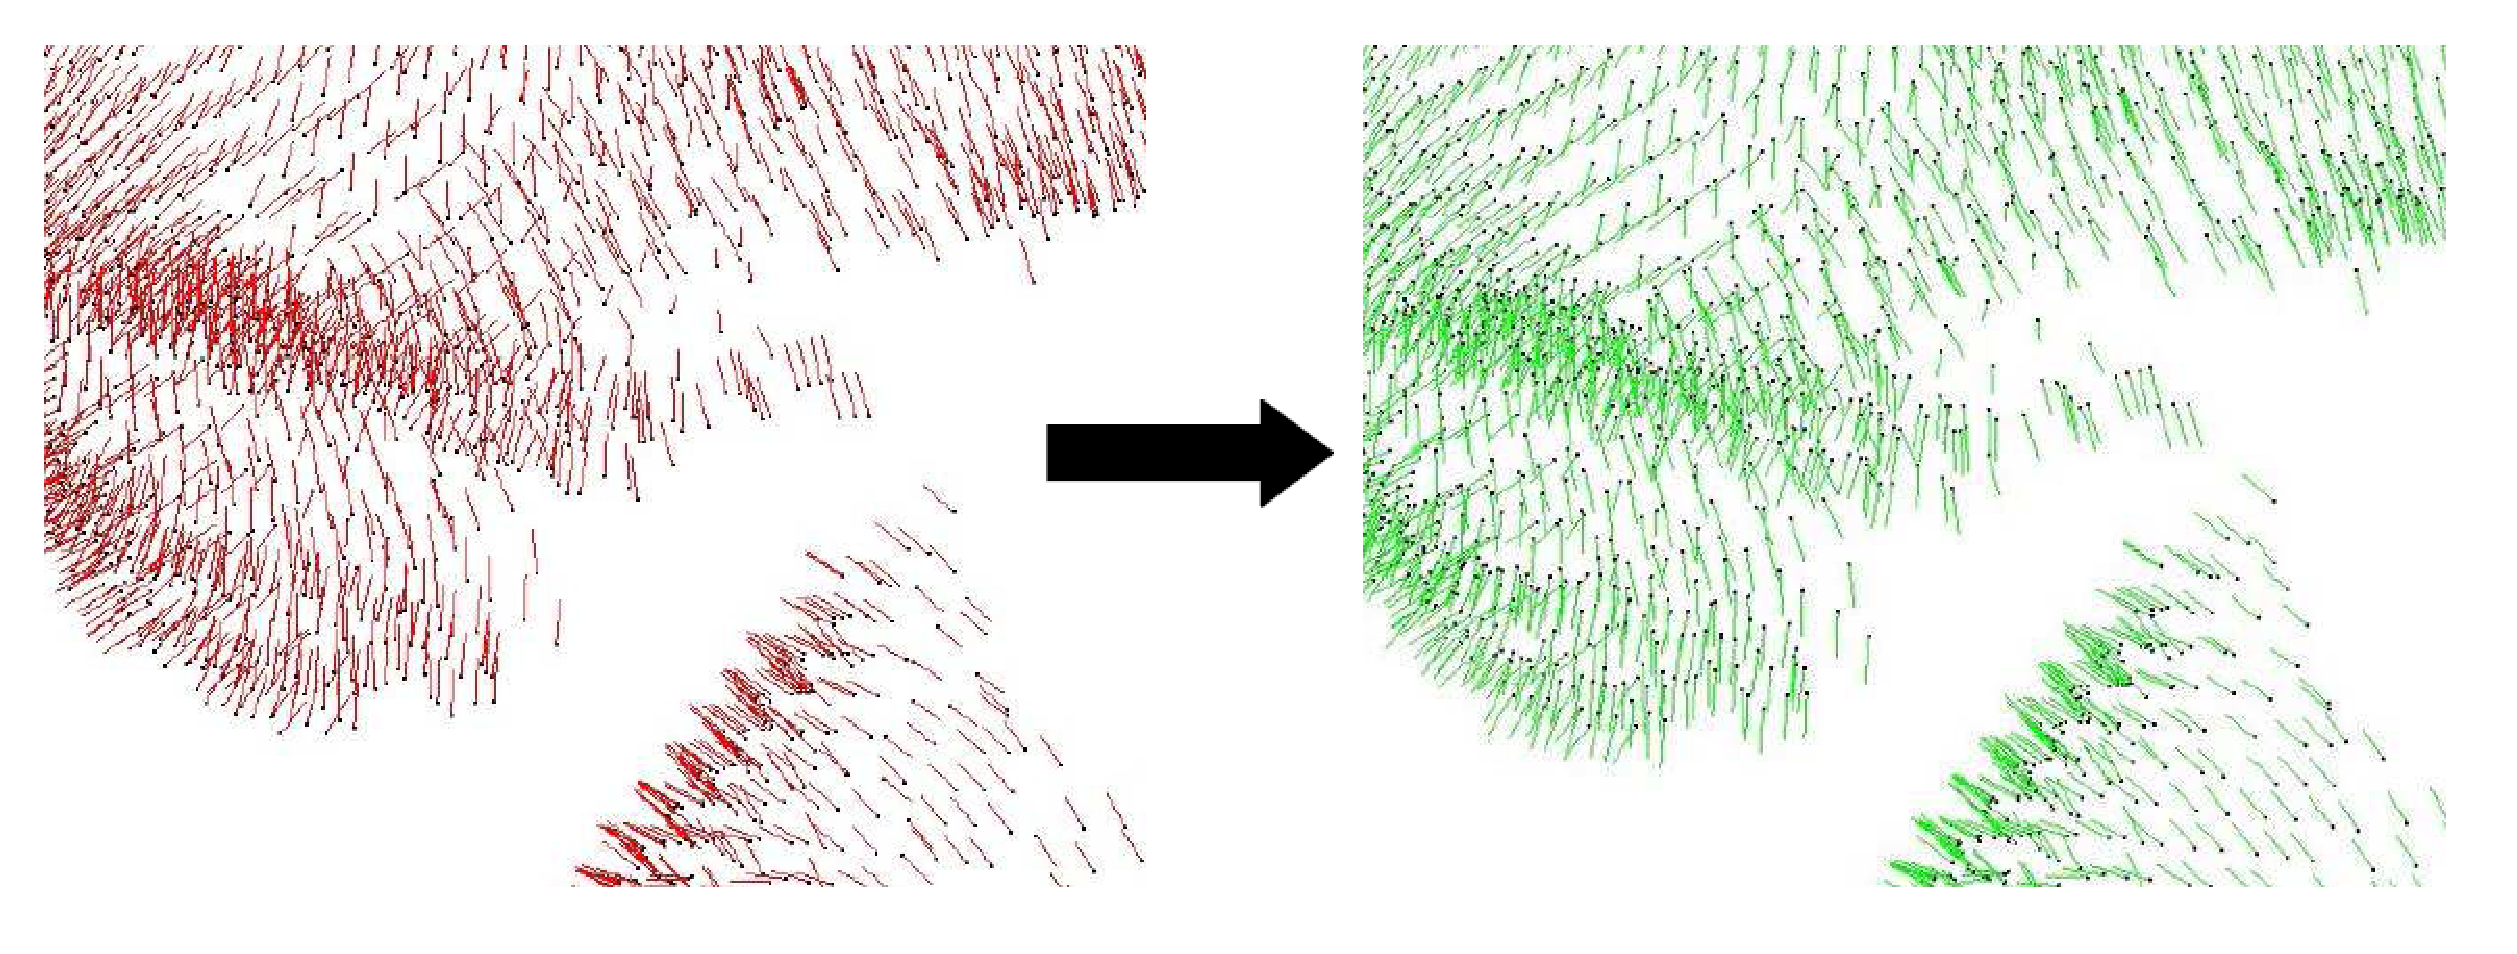
\includegraphics[width=0.9\textwidth]{Surface_reconstruction_3/mst_normal_orientation} % omit .eps suffix
    \end{ccTexOnly}
    \begin{ccHtmlOnly}
        <img width="90%" border=0 src="./mst_normal_orientation.jpg"><P>
    \end{ccHtmlOnly}
    % Title
    \begin{figure}[h]
        \caption{Normal orientation}
    \end{figure}
\end{center}

Example:

See \ccc{pca_normal_estimation_example.cpp} example above.


\subsection{Surface Reconstruction}

\subsubsection{Implicit Functions}

This package implements:

\begin{itemize}
\item Delaunay-based Poisson reconstruction \cite{Kazhdan06}
\item Algebraic Point Set Surfaces \cite{Guennebaud07}
\end{itemize}

\ccRefIdfierPage{CGAL::Poisson_reconstruction_function<GeomTraits, ReconstructionTriangulation_3>}  \\
\ccRefIdfierPage{CGAL::APSS_reconstruction_function<GeomTraits>}  \\

% Insert image APSS.jpg/eps
\begin{center}
    \label{Surface_reconstruction_3-fig-APSS}
    % Image
    \begin{ccTexOnly}
        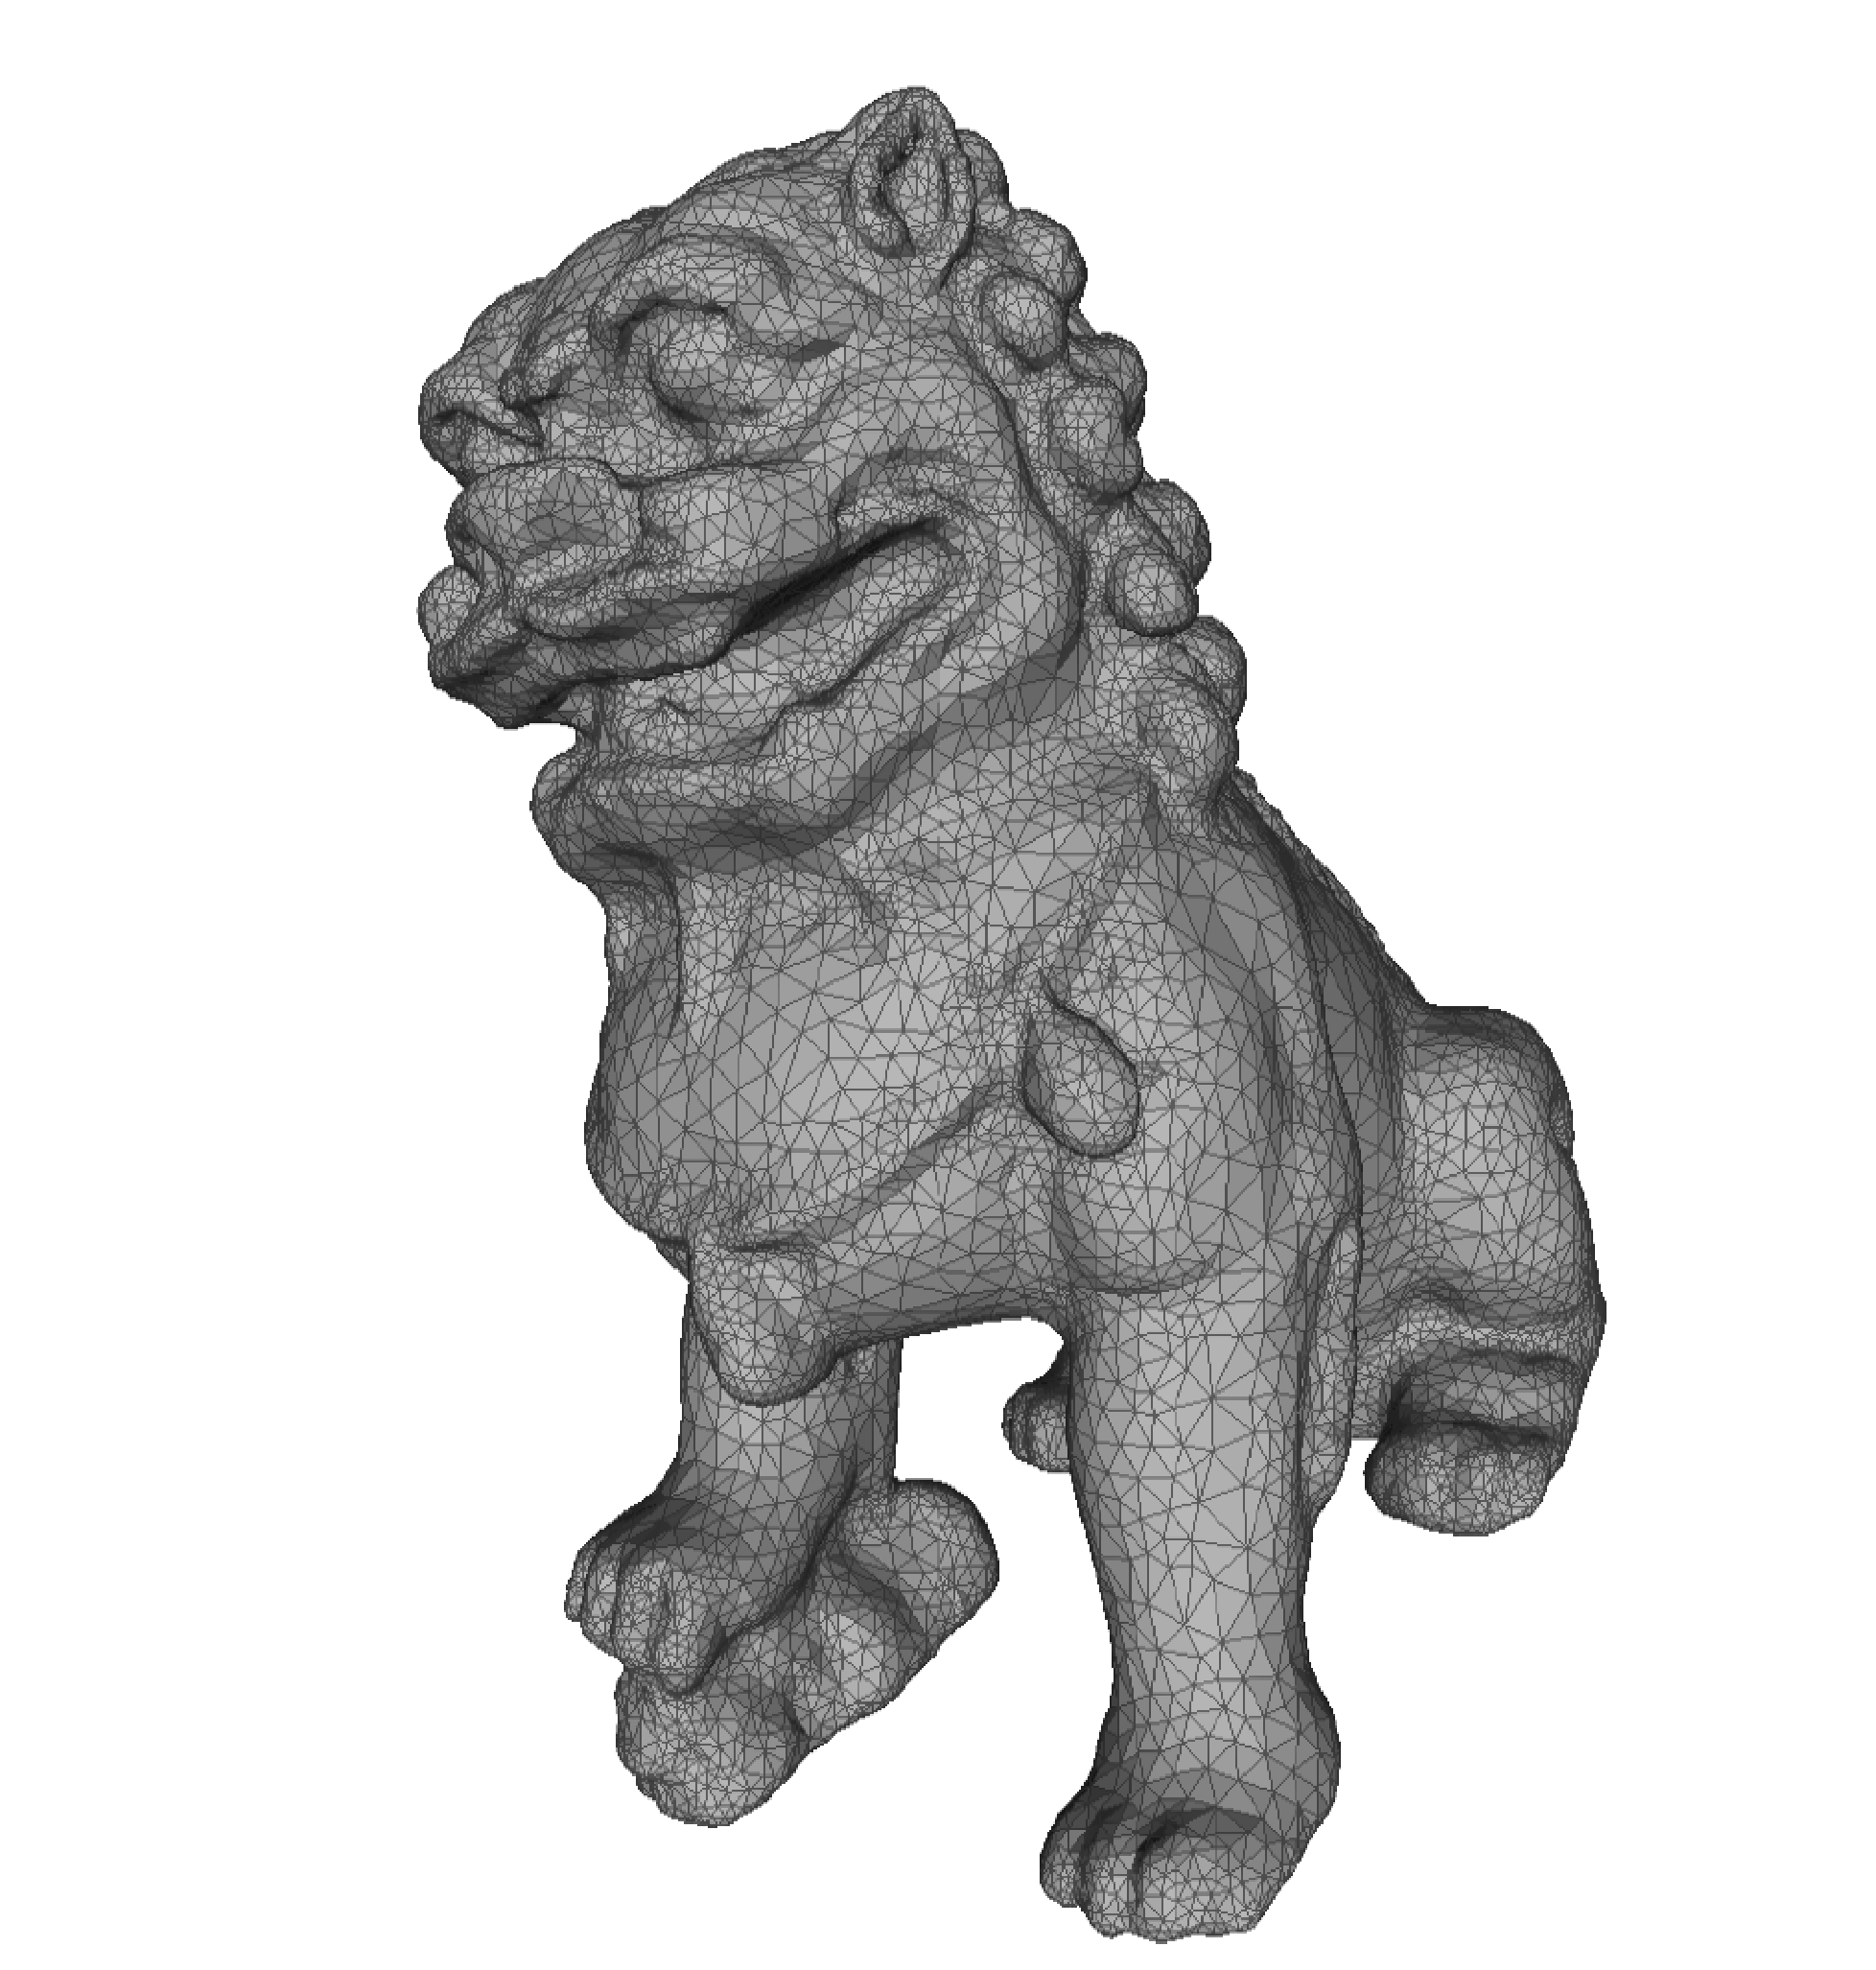
\includegraphics[width=0.5\textwidth]{Surface_reconstruction_3/APSS} % omit .eps suffix
    \end{ccTexOnly}
    \begin{ccHtmlOnly}
        <img width="50%" border=0 src="./APSS.jpg"><P>
    \end{ccHtmlOnly}
    % Title
    \begin{figure}[h]
        \caption{APSS reconstruction}
    \end{figure}
\end{center}


\subsubsection{Implicit Functions Contouring}

Implicit functions can be contoured to reconstruct a surface by:

\begin{itemize}
\item \cgal\ Surface Mesh Generator~\cite{cgal:ry-gsddrm-06,cgal:bo-pgsms-05}
\end{itemize}

\ccRefIdfierPage{CGAL::make_surface_mesh}  \\

The parameter \ccc{Tag} affects the behavior of \ccc{make_surface_mesh()}: \\
- \ccc{Manifold_tag}: the output mesh is guaranteed to be a manifold
surface without boundary.\\
- \ccc{Manifold_with_boundary_tag}: the output mesh is guaranteed to be
manifold but may have boundaries.\\
- \ccc{Non_manifold_tag}: the output mesh will be a polygon soup.

Example:

See \ccc{poisson_reconstruction_example.cpp} example above.


\subsection{Output}

\subsubsection{Point Set Output}

The output of the processing stage is a point set with normals.
For convenience, we provide functions to write point sets to standard file formats:

\begin{itemize}
\item XYZ
\item OFF
\end{itemize}

\ccRefIdfierPage{CGAL::surface_reconstruction_write_off_point_cloud}  \\
\ccRefIdfierPage{CGAL::surface_reconstruction_write_xyz}  \\

Example:

See \ccc{surface_reconstruction_read_write_xyz_example.cpp} example above.


\subsubsection{Surface Output}

The surface reconstructed by \ccc{make_surface_mesh()}
is required to be a model of the concept
\ccc{SurfaceMeshComplex_2InTriangulation_3},
a data structure able to represent a two dimensional
complex embedded in a three dimensional triangulation. \\
\ccc{SurfaceMeshComplex_2InTriangulation_3} defines the methods to traverse the reconstructed surface.

As examples, we provide functions to:

\begin{itemize}
\item write the reconstructed surface to standard OFF file format
\item convert the reconstructed surface to a polygon soup
\end{itemize}

\ccRefIdfierPage{CGAL::output_surface_facets_to_off}  \\
\ccRefIdfierPage{CGAL::surface_reconstruction_output_surface_facets}  \\

Example:

See \ccc{poisson_reconstruction_example.cpp} example above.






